\fenicschapter{Dynamic simulations of convection in the Earth's mantle}
              {Thermochemical convection}
              {Lyudmyla Vynnytska,  Stuart R.~Clark and Marie E.~Rognes}
              {vynnytska}

In this chapter, we model dynamic convection processes in the Earth's
mantle; linking the geodynamical equations, numerical implementation and
Python code tightly together. The convection of material is generated by
heating from below with a compositionally distinct and denser layer at
the bottom.  The time-dependent nonlinear partial differential equations
to be solved are the quasi-static Stokes equations with depth- and
temperature-dependent viscosity, and advection-diffusion equations for
the composition and temperature.  We present a numerical algorithm for
the simulation of these equations as well as an implementation of this
algorithm using the DOLFIN Python interface.  The results show that the
compositional heterogeneities persist, but interact strongly with the
convecting system, generating upwellings and movement as material from
the surface displaces them. This chapter will be of interest to those
seeking to model compositional discontinuities using field methods,
as well as those interested in mantle convection simulations.

%------------------------------------------------------------------------------
\section{Convection in the Earth's mantle}

In contrast to the hydrosphere and atmosphere, the Earth's crust and
mantle are primarily solid in nature, allowing the rapid progression
of seismic waves.  However, one of the most important discoveries
of geodynamics is that materials can behave elastically on certain
timescales and viscously on other timescales. Glaciers work on this
principle: solid ice slowly deforms and flows under the effect of gravity.
While glaciers move on the order of meters per day, the mantle moves
at the speed of a few centimeters per year~\citep{vanderMeer2010}.
At this rate, a piece of the Earth's lithosphere, or slab, would take
at least one hundred million years to sink from the Earth's surface to
the outer core~\citep{Jarvis2007}.

Blanketing the outer core, seismologists detect a layer through which
seismic waves are anomalously slow: the D'' (\emph{dee} double prime) layer.
In some regions, this layer is very thin, overlain by fast zones that may
indicate slabs buried deep within the mantle~\citep{McNamaraZhong2005}.
Underneath southern Africa and the Pacific, two prominent seismically
anomalous slow regions exist, seemingly pointing to a hotter or
compositionally denser material~\citep{McNutt1998}. Such heterogeneities
have led geoscientists to speculate on the existence of large chemically
isolated reservoirs in the mantle, perhaps a remnant from the early
Earth's mantle~\citep{Burke2008}.  But how can these chemically
isolated reservoirs survive in a vigorously convecting mantle?
Geodynamicists have tried to answer this question with computer
simulations of thermomechanical convection of a compositionally
heterogeneous mantle; such simulations are more simply termed
thermochemical~\citep{McNamara2010}. The challenge for geodynamicists is:
can the assumptions made in matching the longevity of these reservoirs
be consistent with seismic observations and the physics we know of the
Earth's interior and plate tectonics?

Primarily, the observations we need to match are simply the transfer of
matter between the Earth's interior and surface. At the surface of the
Earth, tectonic plates are bent and pushed into the interior. In other
places, we see large volcanic terranes created by material sourced
from the Earth's mantle. To model the motion of the mantle over long
timescales, the Stokes equations are well established in their ability
to replicate this behavior, given the right assumptions, coupled with
a conservation equation for the thermal energy in the mantle.

%%------------------------------------------------------------------------------

\section{Mathematical statement of the problem}
\label{vynnytska:sec:maths}

We model the problem in a rectangular box $\Omega$ in the Cartesian
coordinate system with coordinates $(x_1, x_2)$, neglecting the
sphericity of the Earth, representing the mantle from the surface to
the core-mantle boundary (see Figure~\ref{vynnytska:fig:IC}). The base
of the box is covered by a relatively thin layer of denser material,
while the initial temperature field is set to represent the colder
lithosphere along the top and slab descending on the right-hand side;
a hotter layer is imposed along the bottom and left to represent the
hotter D'' layer and a plume ascending respectively following the
boundary layer arguments of~\citet{KekenEtAl1997}. The idea is simply
to create an initial configuration that drives the convection of the
problem.
\begin{figure}
   \center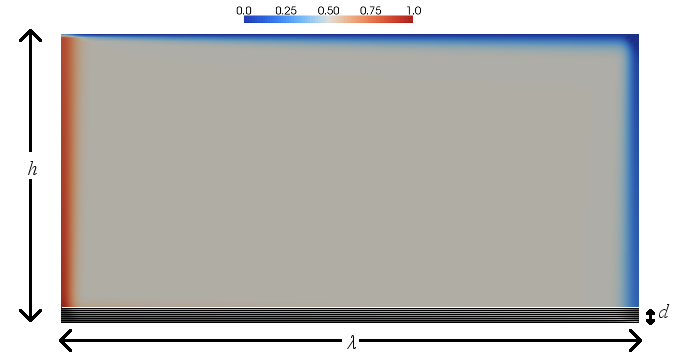
\includegraphics[width=0.95\columnwidth]{chapters/vynnytska/png/layout.png}
    \caption{Initial configuration of the model in the $h$ by
      $\lambda$ rectangular box $\Omega$. Color shows dimensionless
      temperature (for dimensional values, see
      Section~\ref{vynnytska:sec:results}). The shaded layer on the
      bottom with height $d$ is the denser layer corresponding to the
      D'' layer.}
  \label{vynnytska:fig:IC}
\end{figure}

The viscosity of the mantle, on the order of $10^{22} \mathrm{Pa~s}$,
is so high that inertial forces and compressibility are
negligible~\citep{Ricard2009}. If the assumption of compressibility is
relaxed, the lower mantle can support piles of geochemically isolated
material with sharp edges~\citep{TanGurnis2005}. However, for our
purposes, we assume an incompressible thermal flow driven by
temperature and compositional density variations modeled by the
following system of equations:
\begin{align}
  \label{vynnytska:eq:momentum}
  - \Div \sigma^{\prime} - \Grad p
  &=  \left( Rb \, \phi - Ra \, T \right) e,
\\
  \label{vynnytska:eq:incompress}
  \Div u & =  0,
\\
  \label{vynnytska:eq:energy}
  \frac{\partial T}{\partial t} + u \cdot \Grad T & =  \Delta T.
\end{align}
Here, $\sigma^{\prime}$ is the deviatoric stress tensor, $p$
is the pressure, $Ra$ and $Rb$ are the thermal and compositional
Rayleigh numbers, respectively, $T$ is the temperature, $\phi$ is a
composition field, $u$ is the velocity, and $e$ is a unit vector in
the direction of gravity ($-x_2$). Equations given in this section
are nondimensional; scaling and physical constants are presented in
Section~\ref{vynnytska:sec:results}.

The Rayleigh numbers measure the relative importance of buoyancy to
thermal and viscous dissipation ~\citep{KennettBunge2008} given by
thermal diffusivity ($k_{th}$) and the reference viscosity ($\eta_0$),
respectively.  The change in density due to heat is a product of the
thermal contrast ($\Delta T$), thermal expansivity ($\alpha$) and the
reference density ($\rho_0$), while for the composition it is simply
the density contrast ($\Delta \rho$) between the two materials; the
gravitational acceleration ($g$) turns these densities into buoyancies
in the following way:
%%
\begin{equation}
  Ra = \frac{\alpha g \rho_0 \Delta T h^3}{k_{th} \eta_0},  \quad
  Rb = \frac{\Delta \rho g h^3}{k_{th} \eta_0}.
\end{equation}
The Rayleigh numbers, $Ra$ and $Rb$, are defined as equal and as $10^{6}$
within the ranges for the Earth \citep{MontagueKelloggManga1998} and
such that fluid convection dominates.

The mantle flow induces transport of the composition $\phi$. This
transport is governed by the equation
\begin{equation}
  \label{vynnytska:eq:trans}
  \frac{\partial \phi}{\partial t} +  u \cdot \Grad \phi = 0.
\end{equation}
However, some chemical diffusivity $k_{ch}$ is also present in the
physical system~\citep{KekenEtAl1997, HansenYuen1988}. Therefore, we
substitute the pure advection equation~\eqref{vynnytska:eq:trans} by
an advection-diffusion equation of the form
\begin{equation}
  \label{vynnytska:eq:transdif}
  \frac{\partial \phi}{\partial t}
  + u  \cdot \Grad \phi =  k_c \Delta \phi.
\end{equation}
Here, $k_c = k_{ch}/k_{th}$.

It remains to specify the constitutive relationship relating the
deviatoric stress tensor $\sigma^{\prime}$ to the other
variables. Here, we consider the case of a Newtonian rheology with a
depth- and temperature-dependent viscosity
$\eta$~\citep{BlankenbachBusse1989}. The stress-strain relationship is
then described by the equations
\begin{align}
  \sigma^{\prime} &= 2 \eta \dot{\varepsilon} (u),
\\
  \dot{\varepsilon}(u) &= \frac{1}{2} \left (\Grad u + \Grad u^{\top} \right),
\\
  \eta &= \eta(T, x_2) = \eta_0 \exp \left( -b T/\Delta T + c (h - x_2)/ h \right) .
\end{align}
Here, $\dot {\varepsilon}$ is the strain rate tensor, $\eta_0$ is (still)
the reference viscosity, and $b$ and $c$ are given additional parameters.

For the current scenario, we will consider the following boundary
conditions. For the Stokes equations~\eqref{vynnytska:eq:momentum}, we
apply no slip conditions on the bottom boundary ($x_2 = 0$), and free
slip and reflective symmetry on the remaining boundary $\Gamma
= \partial \Omega \backslash \{x: x_2 = 0 \}$:
\begin{equation}
  \label{vynnytska:eq:bcs}
  u |_{x_2 = 0} = 0, \quad
  u_n|_{\Gamma}  =  \sigma^{\prime}_{n \tau} |_{\Gamma} = 0,
\end{equation}
where $n$ is the outward normal and $\tau$ is the tangent vector on
the boundary $\partial \Omega$. For the temperature, we fix its value
on the top and bottom boundary and apply symmetry conditions (or no
heat exchange) on the left- and right-hand boundaries:
\begin{equation}
  T |_{x_2 = 0} = \Delta T, \quad T |_{x_2 = h}  = 0, \quad
  \partial_{x_1} T |_{x_1 = 0}  = \partial_{x_1} T |_{x_1 = \lambda} = 0.
\end{equation}
For the composition $\phi$, we set
\begin{equation}
  \phi |_{x_2 = 0} = 1, \quad \partial_{n} \phi|_{\Gamma} = 0.
\end{equation}
That is, we fix the composition on the bottom of the box $\Omega$
and apply zero flux conditions on the remainder of the boundary. This
condition can be viewed as a consequence of the no outflow conditions
for the velocity.

The initial temperature field is given by $T_0$ (see
Figure~\ref{vynnytska:fig:IC}).  In the below equations, we
give an analytical expression for $T_0$ based on boundary layer
theory~\citep{KekenEtAl1997}, taking the value of $Ra$ with input from
the upper $T_u$, lower $T_l$, right $T_r$ and left $T_s$ parts of the
domain into account:
\begin{align}
    T_0 &= T_u + T_l + T_r + T_s - 1.5,
\\
  q &= \frac{\lambda^{7/3}}{\left(1 + \lambda^4 \right)^{2/3}} \left( \frac{Ra}{2 \sqrt{\pi}}\right)^{2/3},
\\
  Q & = 2\sqrt{\frac{\lambda}{\pi q}},
\\
    T_u &= 0.5 \mathrm{erf} \left( \frac{1-x_2}{2} \sqrt{\frac{q}{x_1}  } \right),
\\
    T_l &= 1 - 0.5 \mathrm{erf} \left( \frac{x_2}{2} \sqrt{\frac{q}{\lambda - x_1}  } \right),
\\
    T_r &= 0.5 + \frac{Q}{2\sqrt{\pi}} \sqrt{\frac{q}{x_{2} + 1} } \mathrm{expc} \left( - \frac{x_1^2 q}{4 x_2 + 4} \right),
\\
    T_s &= 0.5 - \frac{Q}{2\sqrt{\pi}} \sqrt{\frac{q}{2 - x_{2}} } \mathrm{expc} \left( - \frac{ \left(\lambda - x_1 \right)^2  q}{8 - 4 x_2} \right).
\end{align}
In order to keep the initial temperature distribution in the range
between zero and one, we perform an additional correction. According
to the above equations there are two peaks: positive in the top
right and negative in the bottom left corners. We mapped all values
below zero to zero and above one to one. The initial composition
$\phi$ is a step function equal to one on the bottom layer and to zero
on the top layer.

%%------------------------------------------------------------------------------

\section{Numerical method}

In this section, we present a numerical solution method for the
thermochemical convection model established in the previous. Instead
of solving the fully coupled system of nonlinear time-dependent partial
differential equations, we consider a predictor-corrector based splitting
scheme~\citep{BergKekenYuen1993, HansenEbel1988}. In view of this, we
present numerical methods for the solution of each separate equation
before formulating the complete algorithm. Special attention must be
paid to the discretization of the energy~\eqref{vynnytska:eq:energy}
and transport equations~\eqref{vynnytska:eq:transdif}
due to the temperature gradient and the interface
between the compositionally distinct layers. For the Stokes
equations~\eqref{vynnytska:eq:momentum}~--~\eqref{vynnytska:eq:incompress},
we use a mixed finite element formulation, thus obtaining solutions for
the velocity and pressure simultaneously.


\subsection{Mixed finite element formulation of the Stokes equations}

Let $\mathcal{T}_h = \{T\}$ be a mesh\footnote{Note that $T$ is used
to denote an element (cell) in a mesh in this section, in addition to
being used to denote the continuous temperature field $T$.} of the
domain $\Omega$. Let $V_h$ and $Q_h$ be finite dimensional spaces,
defined relative to the mesh $\mathcal{T}_h$, for the velocity and
pressure fields, respectively. The standard discrete mixed finite
element formulation with independent approximation of the (continuous)
velocity field $u$ and the pressure field $p$ for the incompressible
Stokes
equations~\eqref{vynnytska:eq:momentum}~--~\eqref{vynnytska:eq:incompress}
with the boundary conditions given by~\eqref{vynnytska:eq:bcs} reads
as follows: for a given temperature $T_h$ and composition $\phi_h$,
find $u_h \in V_h$ and $p_h \in Q_h$ such that
\begin{equation}
  \label{vynnytska:eq:mixed}
  a_{IS} ( (u_h, p_h), (v_h, q_h) ) = L_{IS} ( (v_h, q_h) )
\end{equation}
for all $v_h \in V_h$ and all $q_h \in Q_h$, where
\begin{align}
  a_{IS} ( (u_h, p_h), (v_h, q_h) )
  & = \int_{\Omega} 2 \eta \dot {\varepsilon}(u_h)  \cdot \dot {\varepsilon}(v_h)
  + p_h \Div v_h + q_h \Div u_h \dx,
\\
  L_{IS} ( (v_h, q_h) ) &=
  \int_{\Omega} ( Ra T_h - Rb \phi_{h} ) e \cdot v_h  \dx.
\end{align}
In the subsequent simulations, we use the lowest order Taylor--Hood
elements for the velocity and the pressure; that is, the combination
of continuous piecewise quadratic vector fields for $V_h$ and
continuous piecewise linears for $Q_h$~\citep{TaylorHood1973}.

\subsection{Discontinuous Galerkin formulation of advection--diffusion equations}

The energy and transport equations~\eqref{vynnytska:eq:energy}
and~\eqref{vynnytska:eq:transdif} have the same structure from the
mathematical point of view. The equations both model the time
evolution of advection-diffusion processes, allowing the numerical
analysis to be performed by the same numerical scheme. However, the
numerical treatment of advection dominated advection--diffusion
equations is nontrivial. There exists a large body of research on the
development of efficient computational schemes for such kinds of
problems~\citep{Lin2006, ZienkiewiczTaylor2000}.  Within the finite
element setting, there are two main approaches: Petrov-Galerkin
approximation and discontinuous Galerkin methods. Here, we prefer a
discontinuous Galerkin method because it deals effectively with
discontinuous property fields. In the following, we describe an
upwinded discontinuous Galerkin formulation for the
equation~\eqref{vynnytska:eq:transdif} for the compositional field
$\phi$. This formulation also applies for the energy
equation~\eqref{vynnytska:eq:energy} with $k_c = 1$. For the sake of
clarity, we consider the discretization of~\eqref{vynnytska:eq:trans}
separately first.

Using full upwind numerical flux and taking into consideration that
the normal component of the velocity is equal to zero on the boundary, the
spatial, discontinuous finite element discretization
of~\eqref{vynnytska:eq:trans} with a given $u_h$ reads
as~\citep{PietroLoForteParolini2006}: find $\phi_h \in P_h$ such that
\begin{equation}
  \sum_{T \in \mathcal{T}_h} \int_T \frac{\partial \phi_h}{\partial t} \psi_h
  \dx + a_{A} (u_h; \phi_h, \psi_h) = 0,
\end{equation}
for all $\psi_h \in P_h$, where
\begin{equation}
  \label{vynnytska:eq:dgadv}
   a_{A} (u_h; \phi_h, \psi_h )
   =
   - \sum_{T \in \mathcal{T}_h} \int_T \phi_h u_h \cdot \Grad \psi_h \dx
   + \sum_{e \in \Gamma_i} \int_{e} \left (
   u_h \cdot \jump{\psi_h} \avg{\phi_h} + \frac{1}{2}
   | u_h \cdot n | \jump{\psi_h} \jump{\phi_h} \right ) \ds,
\end{equation}
wherein $\Gamma_i$ denotes the interior edges of $\mathcal{T}_h$. The
jump $\jump{\cdot}$ and average $\avg{\cdot}$ operators on an internal
edge shared by elements $T^{+}$ and $T^{-}$ with outward normals $n^+$
and $n^-$ respectively, are defined for generic scalar fields $\alpha$
and vector fields $\beta$ as
\begin{align}
  \jump{\alpha}&= \alpha^{+} n^{+} + \alpha^{-} n^{-}, \quad
  \jump{\beta}  = \beta^{+} \cdot n^{+} + \beta^{-} \cdot n^{-}, \\
  \avg{\alpha} &= \frac{1}{2} \left( \alpha^{+} + \alpha^{-} \right), \quad
  \avg{\beta}   = \frac{1}{2} \left( \beta^{+} + \beta^{-} \right), \\
  \alpha^{\pm}  &= \alpha |_{T^{\pm}}, \quad
  \beta^{\pm}    = \beta |_{T^{\pm}}.
\end{align}

We now turn to consider the diffusive term
of~\eqref{vynnytska:eq:transdif} separately. Its standard variational form
for a symmetric discontinuous Galerkin discretization with a stabilization
penalty term is given by~\citep{Arnold1982}
\begin{multline}
  \label{vynnytska:eq:dgdiff}
    a_D(\phi_h, \psi_h)
    =
    \sum_{T \in \mathcal{T}_h} \int_T k_c \Grad \phi_h \cdot \Grad \psi_h \dx
    + \sum_{e \in \Gamma_i }
    \int_{e} - \avg{k_c \Grad \phi_h} \cdot \jump{\psi_h} \ds
\\
    + \sum_{e \in \Gamma_i} \int_{e} \left(
    - \{ k_c \Grad \psi_h\} \cdot \jump{\phi_h}
    + \frac{\alpha_h k_c}{h_T} \jump{\phi_h} \cdot \jump{\psi_h}
    \right) \ds,
\end{multline}
where $\alpha_h$ is a sufficiently large constant to ensure stability, and
$h_T$ is the size of element~$T$. Combining~\eqref{vynnytska:eq:dgadv}
and~\eqref{vynnytska:eq:dgdiff}, we obtain the following
spatially discrete variational formulation of the transport
equation~\eqref{vynnytska:eq:transdif}: find $\phi_h \in P_h$ such that
\begin{equation}
  \label{vynnytska:eq:semi_composition}
  \sum_{T \in \mathcal{T}_h} \int_T \frac{\partial \phi_h}{\partial t}\psi_h \dx
  + a_{A} (u_h; \phi_h, \psi_h) + a_D(\phi_h, \psi_h) = 0
\end{equation}
for all $\psi_h \in P_h$, where $P_h$ is a finite element space of
discontinuous piecewise polynomial fields, and correspondingly for the
temperature $T_h$. In the subsequent simulations, we will let $P_h$ be
the space of (discontinuous) piecewise linears defined relative to the
mesh $\mathcal{T}_h$.

\subsection{A decoupling predictor-corrector scheme}

Instead of solving the fully coupled nonlinear system of equations
defined
by~\eqref{vynnytska:eq:momentum}~--~\eqref{vynnytska:eq:incompress},
\eqref{vynnytska:eq:energy}, and~\eqref{vynnytska:eq:transdif}, we
use a splitting scheme. In particular, we consider a
predictor--corrector scheme~\citep{BergKekenYuen1993, HansenEbel1988}
for the temperature $T$ in combination with a filtering algorithm for
the composition $\phi$. The filtering algorithm is aimed at correcting
the compositional field from numerical diffusion and dispersion
errors, and is motivated and described in detail
by~\citet{LenardicKaula1993}.

Before outlining the algorithm, we make some comments on the temporal
discretization of~\eqref{vynnytska:eq:semi_composition}
and the corresponding equation for the
temperature. Rewriting~\eqref{vynnytska:eq:semi_composition} as
\begin{equation}
  \frac{\partial r}{\partial t} = W,
\end{equation}
the common $\theta$-scheme for the evolution of $r$ from $r^{k-1}$ to
$r^k$ with time step $\Delta t_k$ reads:
\begin{equation}
  \label{vynnytska:eq:thetascheme}
  \frac{r^k - r^{k-1}}{\Delta t_k} = \theta W^k + (1 - \theta) W^{k-1}.
\end{equation}
The choice $\theta = 1$ corresponds to the backward Euler scheme
while $\theta = 0.5$ corresponds to the Crank--Nicolson scheme. The
predictor--corrector scheme draws on the Crank--Nicolson scheme in using a
two-step procedure. Taking the energy equation for the temperature as an
example, assuming that the temperature at the previous time $T_h^{k-1}$
and the previous velocity $u_h^{k-1}$ are known, the predictor step
computes a predicted temperature $T_h^{pr} \in P_h$ solving the implicit
Euler equations for all $\psi_h \in P_h$:
\begin{equation}
  \label{vynnytska:eq:predictor}
  \sum_{T \in \mathcal{T}_h}
  \int_T \frac{T_h^{pr} - T_h^{k-1}}{\Delta t_k} \psi_h \dx
  + a_{A} (u_h^{k-1}; T_h^{pr}, \psi_h) + a_D (T_h^{pr}, \psi_h) = 0,
\end{equation}
where $a_A$ and $a_D$ are defined by~\eqref{vynnytska:eq:dgadv}
and~\eqref{vynnytska:eq:dgdiff}, respectively. Later, the corrector
step computes the corrected temperature $T_h^k$ by a Crank--Nicolson
scheme
\begin{multline}
  \label{vynnytska:eq:corrector}
    \sum_{T \in \mathcal{T}_h}
    \int_T \frac{T_h^k - T_h^{k-1}}{\Delta t_k} \psi_h \dx
    + 0.5 \left( a_{A} (u_h^{pr}; T_h^{k}, \psi_h)
    + a_D (T_h^{k}, \psi_h) \right)
\\
    + 0.5 \left( a_{A} (u_h^{k-1}; T_h^{k-1}, \psi_h)
    + a_D (T_h^{k-1}, \psi_h) \right) = 0,
\end{multline}
but using a predicted velocity $u_h^{pr}$, which will be further
specified in Algorithm~\ref{vynnytska:alg:algorithm}
below.
\begin{algorithm}
  \begin{tabbing}
    Initialize temperature $T^0$ and composition $\phi^0$. \\
    Compute initial velocity $u^0$ by
    solving~\eqref{vynnytska:eq:mixed} with $T^0$ and $\phi^0$. \\
    Compute time step $\Delta t_1$ from $u^0$ according
    to~\eqref{vynnytska:eq:timestep}. \\
    \textbf{for}  {$k = 1, \dots, n$}. \\
    \tab (1) Solve~\eqref{vynnytska:eq:predictor} to obtain $T_h^{pr}$. \\
    \tab (2) Solve (the composition equivalent
    of)~\eqref{vynnytska:eq:predictor} to obtain $\phi_h^{pr}$. \\
    \tab (3) Filter predicted composition $\phi_h^{pr}$ to
    obtain $\phi_h^{k}$. \\
    \tab (4) Solve~\eqref{vynnytska:eq:mixed} with $T_h^{pr}$ and
    $\phi_h^{k}$ as input to obtain $u_h^{pr}$. \\
    \tab (5) Solve~\eqref{vynnytska:eq:corrector} to obtain $T_h^{k}$. \\
    \tab (4) Solve~\eqref{vynnytska:eq:mixed} with $T_h^{k}$ and
    $\phi_h^{k}$ as input to obtain $u_h^{k}$. \\
    \tab (6) Compute new time step $\Delta t_{k+1}$ according
    to~\eqref{vynnytska:eq:timestep}. \\
    \textbf{end for}
  \end{tabbing}
  \caption{A predictor--corrector algorithm}
  \label{vynnytska:alg:algorithm}
\end{algorithm}

In order to satisfy a CFL-type stability condition, a variable time
step will be used. In particular, we define each time step $\Delta
t_k$ by the formula
\begin{equation}
   \label{vynnytska:eq:timestep}
   \Delta t_k =  C_{\mathrm{CFL}} h_{\min} / \max{|u^{k-1}_h|},
\end{equation}
where $h_{\min}$ is the minimum cell size of the mesh and
$C_{\mathrm{CFL}}$ is a chosen positive number.

The basic idea of the filtering algorithm is to ensure that $\phi$
remains within the bounds $0 \leqslant \phi \leqslant 1$, and to minimize
dispersion error.  We refer the reader to~\citet{LenardicKaula1993}
for the detailed explanation and here give the outline of the algorithm
for a discrete property field $\phi = \{\phi_i \}$.
\begin{algorithm}
  \begin{tabbing}
  (1) Compute initial sum $S_0$ of all values of $\phi$. \\
  (2) Find minimal value $\phi_{\min}$ below 0. \\
  (3) Find maximal value $\phi_{\max}$ above 1. \\
  (4) Assign to $\phi_i \leqslant | \phi_{\min} |$ value 0. \\
  (5) Assign to $\phi_i \geqslant 2 - \phi_{\max} $ value 1. \\
  (6) Compute sum $S_1$ of all values of $\phi$. \\
  (7) Compute the number $num$ of $0 < \phi_j < 1$. \\
  (8) Add $dist = (S_1 - S_0)/num$ to all $ 0 < \phi_j < 1$.
  \end{tabbing}
  \caption{A property filtering algorithm}
  \label{vynnytska:alg:filtering}
\end{algorithm}

%%------------------------------------------------------------------------------

\section{Implementation}

\subsection{Main algorithm}

The main body of the implementation consists of the temporal loop
defined in Algorithm~\ref{vynnytska:alg:algorithm}. An abridged version
of this code is listed in Figure~\ref{vynnytska:fig:mainalgorithm},
and explained in detail in the corresponding caption.  As the filtering
step is straightforward to implement based on the algorithm described in
Algorithm~\ref{vynnytska:alg:filtering}, we will not comment any further
on this aspect. Below, we make some general observations and comments.
\begin{itemize}
\item
  In each iteration, five variational problems are solved. First, a
  predicted temperature is computed based on the velocity and the
  temperature from the previous time step. Next, a tentative
  composition is computed based on the velocity and the composition
  from the previous time step; then filtered using as described by
  Algorithm~\ref{vynnytska:alg:filtering}. With the filtered
  composition and the predicted temperature, the velocity and pressure
  are predicted.  The corrected temperature is then calculated by the
  Crank--Nicolson system using the predicted velocity, and the
  velocity and the temperature from the previous time step. The Stokes
  system is then solved again, this time with the filtered composition
  and the corrected temperature as input to yield the corrected
  velocity and pressure at this time step.
\item
  The advection-diffusion problems for calculating the predicted
  composition and the predicted and corrected temperature depend on
  the velocity at the previous and current time steps. Analogously,
  the Stokes equations for the predicted and corrected velocity depend
  on the composition and temperature through the viscosity and the
  source terms. Thus, the linear systems of equations have to be
  assembled (and solved) at each time. For simplicity, we generate the
  variational forms describing the equations and define a
  new \emp{VariationalProblem} for each of these problems at each
  time. The compute time used for this is insignificant in comparison
  with the time required for the assembly and solution of the linear
  systems.
\item
  The linear systems resulting from the equations for the composition
  and the temperature are positive definite but not symmetric. Hence,
  these are solved iteratively using a standard generalized minimal
  residual solver (GMRES). For the simulations considered in the
  subsequent section, these solvers converge in $4 - 10$ iterations.
  On the other hand, the linear systems resulting from the Stokes
  equations are symmetric but indefinite. Non-preconditioned iterative
  solvers typically fail to converge for such systems, while direct
  solvers are prohibitively (memory) expensive. Therefore, these
  systems require preconditioning. Following
  Chapter~\ref{chap:mardal-4}, we here take advantage of a standard
  Stokes preconditioner, neglecting possible advantages in using a
  preconditioner that varies synchronously with the viscosity.  As
  such, we can assemble the preconditioner matrix outside the loop and
  reuse it and the Krylov solver in each iteration.
\item
  The time step \emp{dt} is computed adaptively in each iteration of
  the temporal loop using the
  formula~\eqref{vynnytska:eq:timestep}. The minimal mesh size is
  easily extracted using \emp{mesh.hmin()} and the maximal value for
  the velocity is extracted as the maximal degree of freedom from
  the \emp{numpy} array of degrees of freedom. Since the time step
  varies in each iteration and with the mesh size, it is convenient to
  use a \emp{Constant} for its representation in order to avoid
  recompilation of the variational forms at each iteration.
\item
  The solutions for the composition, the temperature and the velocity
  are stored at each time using the \emp{TimeSeries} class; allowing
  for easy storage and retrieval of meshes and solution
  vectors. Moreover, it naturally encourages a decoupling of the
  simulation and the post-processing of the simulation data. This can
  be highly advantageous, especially for computations with significant
  run-times.
\end{itemize}
In the subsections below, we discuss the definition of each of the
variational forms and problems and an implementational structure for
these.

\begin{figure}
  \begin{center}
    \begin{python}
# Functions at previous time step (and initial conditions)
(phi_, T_, u_, P) = compute_initial_conditions()

# Containers for storage
velocity_series = TimeSeries("bin/velocity")
temperature_series = TimeSeries("bin/temperature")
composition_series = TimeSeries("bin/composition")

# Solver for the Stokes systems
solver = KrylovSolver("tfqmr", "amg_ml")
...
while (t <= finish):

    # Solve for predicted temperature
    (a, L) = energy(mesh, Constant(dt), u_, T_)
    eq = VariationalProblem(a, L, T_bcs)
    eq.parameters["solver"]["linear_solver"] = "gmres"
    eq.solve(T_pr)

    # Solve for predicted phi
    (a, L) = transport(mesh, Constant(dt), u_, phi_)
    eq = VariationalProblem(a, L, bc)
    eq.parameters["solver"]["linear_solver"] = "gmres"
    eq.solve(phi_pr)

    # Filter predicted phi (in place)
    filter_properties(phi_pr)
    phi.assign(phi_pr)

    # Solve for predicted velocity
    H = Ra*T_pr - Rb*phi_pr
    eta = viscosity(T_pr)
    (a, L, precond) = stokes(mesh, eta, H*g)
    (A, b) = assemble_system(a, L, bcs)
    solver.set_operators(A, P)
    solver.solve(velocity_pressure.vector(), b)
    u_pr.assign(velocity_pressure.split()[0])

    # Solve for corrected temperature T
    (a, L) = energy_correction(mesh, Constant(dt), u_pr, u_, T_)
    eq = VariationalProblem(a, L, T_bcs)
    eq.parameters["solver"]["linear_solver"] = "gmres"
    eq.solve(T)

    # Solve for corrected velocity
    H = Ra*T - Rb*phi
    eta = viscosity(T)
    (a, L, precond) = stokes(mesh, eta, H*g)
    (A, b) = assemble_system(a, L, bcs)
    solver.set_operators(A, P)
    solver.solve(velocity_pressure.vector(), b)
    u.assign(velocity_pressure.split()[0])

    # Store stuff
    composition_series.store(phi.vector(), t)
    temperature_series.store(T.vector(), t)
    velocity_series.store(u.vector(), t)

    # Define dt based on CFL condition
    dt = compute_timestep(u)

    # Move to new timestep, including updating functions
    phi_.assign(phi)
    T_.assign(T)
    u_.assign(u)
    t += dt
    \end{python}
  \end{center}

    \caption{Abridged code for the main predictor-corrector algorithm,
      see Algorithm~\ref{vynnytska:alg:algorithm}. The initialization
      of the mesh \emp{mesh}, the viscous and chemical parameters and
      the boundary conditions are omitted. The solution fields are
      consistently named \emp{T}, \emp{u}, and \emp{phi} for
      solutions at the current time; \emp{T\_}, \emp{u\_},
      and \emp{phi\_} for fields at the previous time;
      and \emp{T\_pr}, \emp{u\_pr}, and \emp{phi\_pr} for predictor
      fields. These \emp{Functions} are all initialized (but the
      initialization is not included here).
%
      First, the initial conditions are constructed. This involves the
      solution of a Stokes system for the initial velocity \emp{u\_},
      and in particular the construction of a preconditioner matrix
      \emp{P}. Since the matrix is to be reused, the initial
      condition computation also return this matrix. Next,
      \emp{TimeSeries} objects are initialized for easy storage of
      the solutions at each time. The \emp{KrylovSolver} can also be
      reused in each iteration and is therefore created outside the
      loop.
%
      The contents of the loop follow steps (1) -- (6) of
      Algorithm~\ref{vynnytska:alg:algorithm}. First, the predicted
      temperature \emp{T\_pr} must be computed. This is done is 4
      substeps: the forms for the variational problem are created;
      the forms are passed together with the boundary conditions to a
      \emp{VariationalProblem}; the type of linear solver is set for
      the problem; and the problem is solved. Next, the same steps are
      performed for the predicted composition \emp{phi\_pr}. The
      predicted composition is then filtered (in place) and also
      assigned to \emp{phi}.
%
      Using the predicted temperature and filtered composition, the
      source term and viscosity for the Stokes equations are defined,
      and then the variational Stokes form is created. In order to
      retain the symmetry of the matrix under the application of
      Dirichlet boundary conditions, the linear system is assembled
      and solved explicitly. This consists of calling the method
      \emp{assemble\_system}, updating the \emp{KrylovSolver} with
      the current operators \emp{A} and \emp{P}, and applying the
      solver to the right-hand side vector. The procedure is repeated
      for the corrected temperature and again for the corrected Stokes
      system.
%
      Finally, the solution fields at the current time are stored, the
      new time step \emp{dt} is computed based on the current velocity
      and the current solutions are assigned to the previous time as
      we step forward in time.}
  \label{vynnytska:fig:mainalgorithm}
\end{figure}

\subsection{Variational formulation of the Stokes equations}

The mixed variational formulation for the Stokes equations is
classical and listed in Figure~\ref{vynnytska:fig:stokes}. The
definition of the bilinear and linear forms rely only on the mesh, a
source vector field $f$ = $(Ra T_h - Rb \phi_h) e$ and the viscosity
$\eta$, see~\eqref{vynnytska:eq:mixed}.  The viscosity itself is
temperature- and depth-dependent, but crucially not velocity
dependent.  Thus the bilinear and linear forms can be represented by
standard linear formulations.  Since the preconditioner for this
system relies on the same function spaces and basis functions, we
define the form for the preconditioner together with the variational
forms describing the partial differential equation.
\begin{figure}
  \begin{python}
def stokes(mesh, eta, f):

    # Define spatial discretization (Taylor--Hood)
    V = VectorFunctionSpace(mesh, "CG", 2)
    Q = FunctionSpace(mesh, "CG", 1)
    W = V * Q

    # Define basis functions
    (u, p) = TrialFunctions(W)
    (v, q) = TestFunctions(W)

    # Define equation F((u, p), (v, q)) = 0
    F = (2.0*eta*inner(sym(grad(u)),sym(grad(v)))*dx
         + div(v)*p*dx
         + div(u)*q*dx
         + inner(f, v)*dx)

    # Define form for preconditioner
    precond = inner(grad(u), grad(v))*dx + p*q*dx

    # Return right and left hand side
    # and preconditioner
    return (lhs(F), rhs(F), precond)
  \end{python}

  \caption{Definition of variational forms for the Stokes equations
    and the corresponding preconditioner. The Taylor--Hood mixed
    finite element space is defined by combining Lagrange vector
    elements of polynomial order 2 with Lagrange elements of order
    1. The equation is phrased in the style $F(\cdot, \cdot) = 0$, and
    the form for the preconditioner is defined using the same basis
    functions. The left- and right-hand side of the form $F$ are
    extracted using the UFL functions \emp{lhs}
    and \emp{rhs}.}
  \label{vynnytska:fig:stokes}
\end{figure}

\subsection{Variational formulation of advection-diffusion equations}

In the implementation of the variational forms for the
advection-diffusion problems, we emphasize the following:
first, the variational forms defining the predictor step for
the temperature and the composition are the same (modulo the
diffusivity constant and possibly the penalty constant).  Second, the
predictor and the corrector steps for the temperature involve the same
mathematical building blocks. Third, discontinuous Galerkin methods
often involve quite a number of terms and the combined forms may
easily become intractable. In view of these aspects, a minimal (as in
highly reused) code close to mathematical syntax seemed preferable.

To this end, the implementation mimics the structure defined
by~\eqref{vynnytska:eq:dgadv},~\eqref{vynnytska:eq:dgdiff}, and
\eqref{vynnytska:eq:thetascheme}. The pure advection form $a_A$ and
the pure diffusion form $a_D$ are defined through separate Python
functions. The code for these is listed in
Figures~\ref{vynnytska:fig:advection}
and~\ref{vynnytska:fig:diffusion} and explained in the captions of
those figures. The implementation of the weak forms of the predictor
equation for the composition, and the predictor and corrector
equations for the temperature are then built using these basic functions. The
code for the corrector equation is included and discussed
in~Figure~\ref{vynnytska:fig:temperaturecorrection}. The code for the
predictor equations is similar but simpler and not discussed
here.
\begin{figure}
  \begin{center}
    \begin{python}
def advection(phi, psi, u, n, theta=1.0):

    # Define |u * n|
    un = abs(dot(u('+'), n('+')))

    # Contributions from cells
    a_cell = -theta*dot(u*phi, grad(psi))*dx

    # Contribution from interior facets
    a_int = theta*(dot(u('+'), jump(psi,n))*avg(phi)
        + 0.5*un*dot(jump(phi, n), jump(psi, n)))*dS

    return a_cell + a_int
    \end{python}
  \end{center}
  \caption{Definition of an upwinded discontinuous Galerkin
    formulation of the advection term. The input consists of:
    \emp{phi} and \emp{psi} (typically functions or basis
    functions); a given velocity \emp{u}; a facet normal \emp{n};
    and an optional scalar multiplier \emp{theta}. The absolute
    value of the normal component of \emp{u} is defined and the
    contributions from the cell integrals and facet integrals are
    defined in accordance with~\eqref{vynnytska:eq:dgadv}. The sum
    of the contributions is returned.}
  \label{vynnytska:fig:advection}
\end{figure}
%
\begin{figure}
  \begin{center}
    \begin{python}
def diffusion(phi, psi, k_c, alpha, n, h, theta=1.0):

    # Contribution from the cells
    a_cell = theta*k_c*dot(grad(phi), grad(psi))*dx

    # Contribution from the interior facets
    a_int = theta*(k_c('+')*alpha('+')/h('+')
                   * dot(jump(phi, n), jump(psi, n))
        - k_c('+')*dot(avg(grad(psi)), jump(phi,n))
        - k_c('+')*dot(jump(psi, n), avg(grad(phi)))
        )*dS

    return a_cell + a_int
    \end{python}
  \end{center}
  \caption{Definition of a discontinuous Galerkin formulation of the
    diffusion term. The input consists of: \emp{phi} and \emp{psi}
    (typically functions or basis functions); the diffusivity
    constant \emp{k\_c}; a stabilization parameter \emp{alpha}; a
    facet normal \emp{n}; the cell size \emp{h}; and an optional
    scalar multiplier \emp{theta}. The contributions from the cell
    integrals and facet integrals are defined
    following~\eqref{vynnytska:eq:dgdiff}. The sum of the
    contributions is returned.}
  \label{vynnytska:fig:diffusion}
\end{figure}

\begin{figure}
  \begin{center}
    \begin{python}
def energy_correction(mesh, dt, u, u_, T_):

    # Define function space and test and trial functions
    P = FunctionSpace(mesh, "DG", 1)
    T = TrialFunction(P)
    psi = TestFunction(P)

    # Diffusivity constant
    k_c = Constant(1.0)

    # Constants associated with DG scheme
    alpha = Constant(50.0)
    h = CellSize(mesh)
    n = FacetNormal(mesh)

    # Define discrete time derivative operator
    Dt = lambda T: (T - T_)/dt

    # Add syntactical sugar for a_A and a_D
    a_A = lambda u, T, psi: \
              advection(T, psi, u, n, theta=0.5)
    a_D = lambda u, T, psi: \
              diffusion(T, psi, k_c, alpha,
                        n, h, theta=0.5)

    # Define form
    F = (Dt(T)*psi*dx
         + a_A(u, T, psi) + a_A(u_, T_, psi)
         + a_D(u, T, psi) + a_D(u_, T_, psi))

    return (lhs(F), rhs(F))
    \end{python}
    \end{center}
    \caption{Definition of variational forms for one correction step
      for the temperature, see~\eqref{vynnytska:eq:corrector}. The
      input is the mesh, the time step \emp{dt}, two given velocities
      \emp{u} and \emp{u\_}, and (typically) a previous temperature
      \emp{T\_}. We define the function space of (discontinuous)
      piecewise linears, the unknown temperature \emp{T} and the test
      function \emp{psi}. The diffusivity constant \emp{k\_c} is in
      this case $1.0$. We define the penalty parameter \emp{alpha}
      and also the cell normal \emp{n} and mesh size \emp{h} to be
      used in the advection and diffusion forms.
%
      We use \emp{lambda} functions to reduce the number of input
      arguments to the advection and diffusion functions. This is in
      part merely syntactical, but does also increase readability and
      facilitates debugging. The input to the functions \emp{a\_A}
      and \emp{a\_D} thus directly corresponds to the arguments of
      $a_A$ and $a_D$.
%
      The equation is again phrased in the style $F(\cdot, \cdot) =
      0$. The reader is encouraged to compare the code with the
      mathematical formulation of the equation,
      see~\eqref{vynnytska:eq:corrector}. Finally, the left- and
      right-hand side forms are extracted using the UFL
      functions \emp{lhs} and \emp{rhs}.}
  \label{vynnytska:fig:temperaturecorrection}
\end{figure}

%%------------------------------------------------------------------------------

\section{Results}
\label{vynnytska:sec:results}

In this section we present the results of the thermochemical
convection simulation, calculated on a mesh constructed by dividing
the domain into $160 \times 80$ squares. Each square is split into two
triangles by the right diagonal. The $C_{\mathrm{CFL}}$ time step
parameter in~\eqref{vynnytska:eq:timestep} is $0.5$.

The equations presented in Section~\ref{vynnytska:sec:maths} are
dimensionalised using the physical parameters in
Table~\ref{vynnytska:table:variables}. Scaling parameters for time
$t_s$ and velocity $u_s$ are obtained as follows:
\begin{align}
 \label{vynnytska:eq:velsc}
 t_s = \frac{h^2}{k_{th}}, \quad u_s = \frac{h}{t_s}.
\end{align}

Convection in the model domain is determined by the
kinematic energy of the fluid, given by:
\begin{align}
  \label{vynnytska:eq:KE}
  E_{K} = \frac{1}{2}\int_{\Omega}\rho \Vert \bm{u} \Vert^{2}dx.
\end{align}
Since the variation in density is small, $\rho$ can be taken out of
the integral, and by defining the root-mean square velocity, $u_{\mathrm{rms}}$
by:
\begin{align}
  \label{vynnytska:eq:u_rms}
  u_{\mathrm{rms}} =\left( \frac{1}{\lambda h} \int_{\Omega} \Vert \bm{u} \Vert^{2} d\bm{x}  \right)^{1/2},
\end{align}
we have the relationship:
\begin{align}
  \label{vynnytska:eq:KEu_rms}
  E_{K} \approx \frac{1}{2} \rho \lambda h u_{\mathrm{rms}}^{2}.
\end{align}
Thus, $u_{\mathrm{rms}}$ is a scaled measure of the kinematic energy of
convection. For the discussion of the results, we will use
Figure~\ref{vynnytska:fig:rms_velocity} to describe the local turning
points, $A$ to $M$, of the root-mean square velocity and refer to the
driving forces in the model to explain these turning points. See the
captions to Figures~\ref{vynnytska:fig:BG} and~\ref{vynnytska:fig:HM}
for details.

\begin{table}
  \begin{tabular}{l c c c}
    & & Dimensional & Dimensionless \\
    Parameter & & value & value \\
    \toprule
    Box height & $h$ & $3000\mathrm{km}$ & $1.0$\\
    Box length & $\lambda$ & $6000\mathrm{km}$ & $2.0$ \\
    Boundary layer thickness & $d$ & $150\mathrm{km}$ & $0.05$ \\
    Acceleration due to gravity & $g$ & $10\mathrm{m/s^2}$ & $1.0$ \\
    Thermal contrast & $\Delta T$ & $3000\mathrm{K}$ & $1.0$ \\
    Thermal expansivity & $\alpha$ & $2 \times 10^{-5}\mathrm{K^{-1}}$ & \\
    Thermal diffusivity & $k_{th}$ & $10^{-6}\mathrm{m^{2}/s}$ & \\
    Chemical diffusivity & $k_{ch}$ & $10^{-10}\mathrm{m^{2}/s}$ & \\
    Reference density & $\rho_{0}$ & $3100\mathrm{kg/m^{3}}$ &  \\
    Compositional density contrast & $\Delta \rho $ & $185\mathrm{kg/m^{3}}$ & $1.0$ \\
    Reference viscosity & $\eta_{0}$ & $5 \times 10^{22} \mathrm{Pa \, s}$ & $1.0$ \\
    Thermal Rayleigh number & $Ra$ & $1 \times 10^{6}$ & $ 1 \times 10^{6}$\\
    Chemical Rayleigh number & $Rb$ & $1 \times 10^{6}$ & $1 \times 10^{6}$\\
    Velocity & $u_s$ & $3 \times 10^{-13} \mathrm{m/s}$& $1.0$ \\
    Time & $t_s$ & $1 \times 10^{19} \mathrm{s}$& $1.0$ \\
    \bottomrule
  \end{tabular}
  \caption{Specification of parameters and parameter values.}
  \label{vynnytska:table:variables}
\end{table}

\begin{figure}
  \center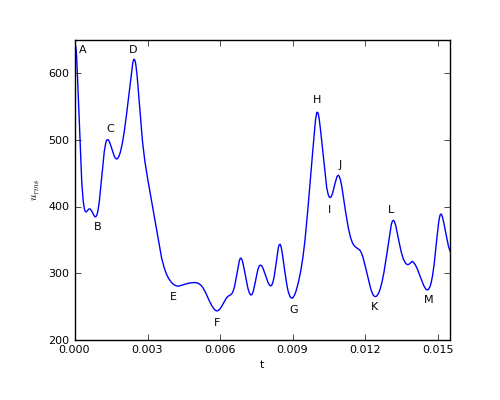
\includegraphics[width=0.95\columnwidth]{chapters/vynnytska/png/u_rms.png}
  \caption{Dimensionless root mean square velocity over
  dimensionless time. $A$ to $M$ are labels used to refer to stages
  in the model. A nondimensional time period of $0.001$ corresponds to
  approximately 300 Ma, and the dimensional value for $u_{\mathrm{rms}} = 100$ is
  approximately $1\,\mathrm{mm/year}$.}
\label{vynnytska:fig:rms_velocity}
\end{figure}

\begin{figure}
\begin{center}
\begin{tabular}{c  r}
Temperature & Viscosity \\
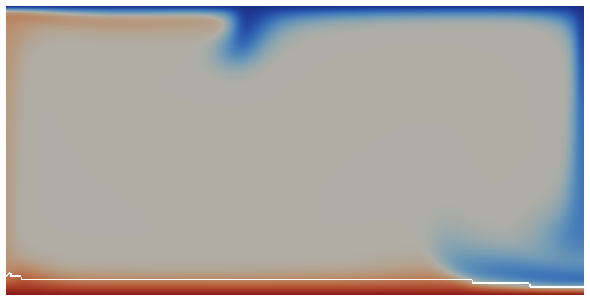
\includegraphics[width=0.45\columnwidth]{chapters/vynnytska/png/tmB.png} &
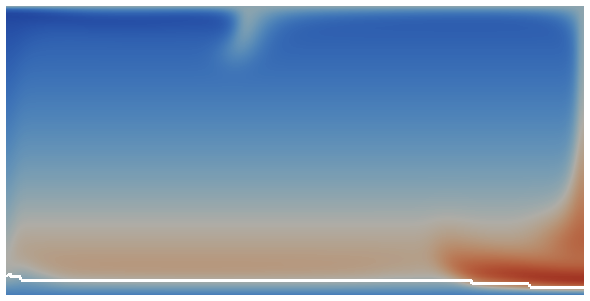
\includegraphics[width=0.45\columnwidth]{chapters/vynnytska/png/visB.png} \\& $B$ \\
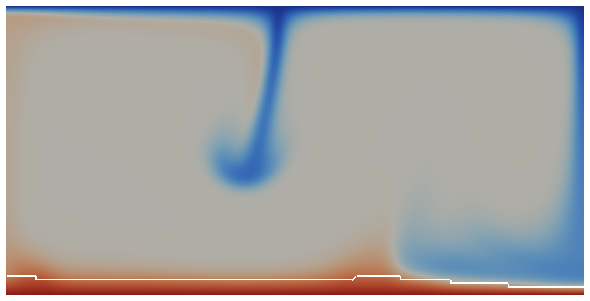
\includegraphics[width=0.45\columnwidth]{chapters/vynnytska/png/tmC.png} &
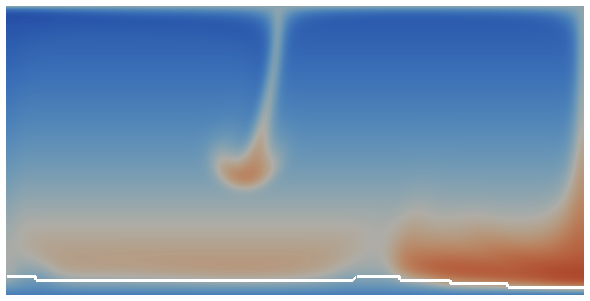
\includegraphics[width=0.45\columnwidth]{chapters/vynnytska/png/visC.png} \\& $C$ \\
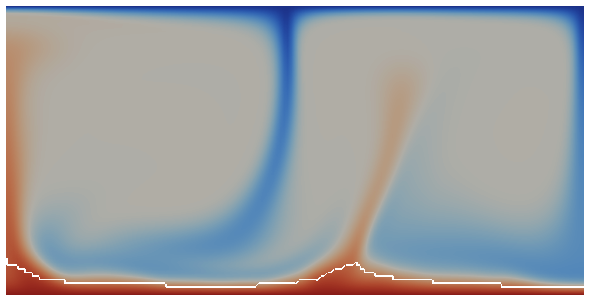
\includegraphics[width=0.45\columnwidth]{chapters/vynnytska/png/tmD.png} &
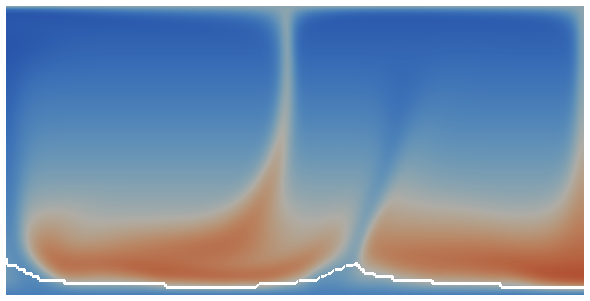
\includegraphics[width=0.45\columnwidth]{chapters/vynnytska/png/visD.png} \\& $D$ \\
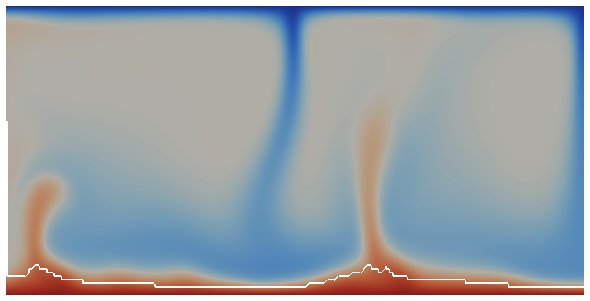
\includegraphics[width=0.45\columnwidth]{chapters/vynnytska/png/tmE.png} &
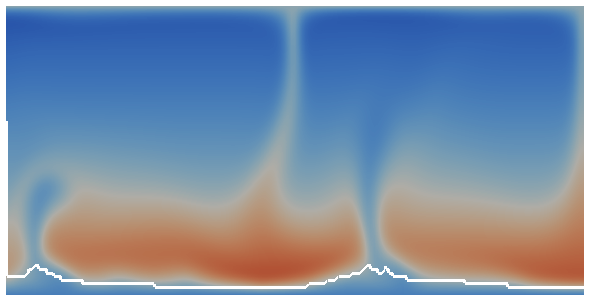
\includegraphics[width=0.45\columnwidth]{chapters/vynnytska/png/visE.png} \\& $E$ \\
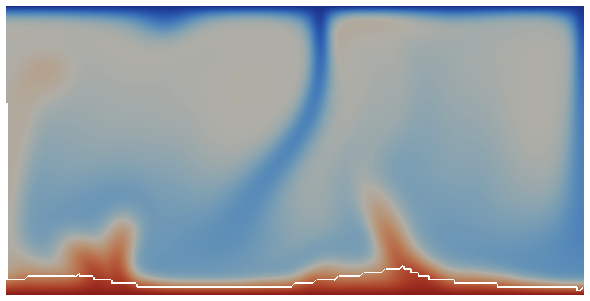
\includegraphics[width=0.45\columnwidth]{chapters/vynnytska/png/tmF.png} &
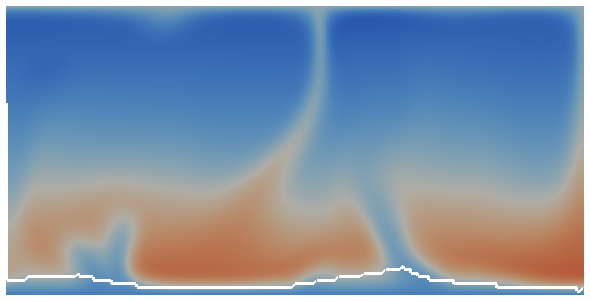
\includegraphics[width=0.45\columnwidth]{chapters/vynnytska/png/visF.png} \\& $F$ \\
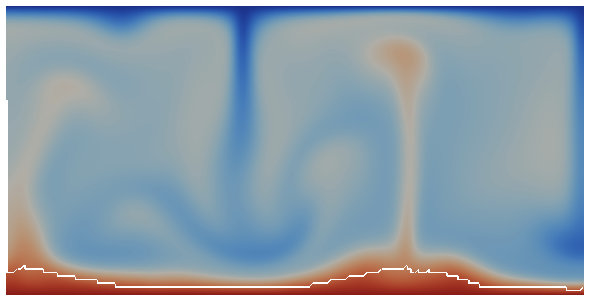
\includegraphics[width=0.45\columnwidth]{chapters/vynnytska/png/tmG.png} &
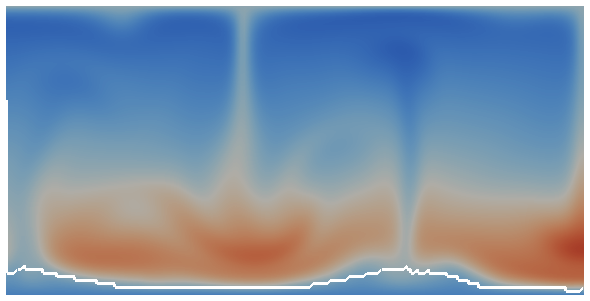
\includegraphics[width=0.45\columnwidth]{chapters/vynnytska/png/visG.png} \\& $G$ \\
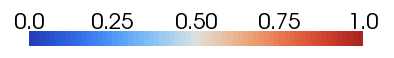
\includegraphics[width=0.45\columnwidth]{chapters/vynnytska/png/tmleg.png} &
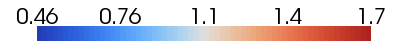
\includegraphics[width=0.45\columnwidth]{chapters/vynnytska/png/visleg.png}
\end{tabular}
\end{center}
\caption{Dimensionless temperature and viscosity for turning points
  $A$ to $G$, with composition barrier shown in white. To convert to physically
  relevant temperature contrast and viscosities,
  these values should be multiplied by dimensional $\eta_0$ and $\Delta T$
  from Table~\ref{vynnytska:table:variables}. The initial
  condition drives the system's high velocity from point $A$, but as
  the cold surface material (slab) reaches the deeper mantle, there is
  a retardation of the flow, towards $B$. The rising hot material
  (plume) during the stage $A$ to $B$ drives lateral flow of the
  surface causing cold material to build up until $B$. From $B$ to $C$
  this cold material begins to rapidly sink, increasing $u_{\mathrm{rms}}$
  until it is slowed by the increasing viscosity at $C$. However, the
  slab's downward motion has created a thermal instability at the base
  of the model, which rises between $C$ and $D$ increasing $u_{\mathrm{rms}}$
  again. The pace of the material slows as the plume necks between $D$
  and $E$ and the compositional density of the remaining material
  prevents it from rising further. A small plume rises from the left
  side of the base, increasing the $u_{\mathrm{rms}}$ briefly. Between $E$ and
  $G$ short-lived plumes and slabs are generated from the bottom and
  top boundary layers, causing small instabilities in the root-mean
  square velocity.}
\label{vynnytska:fig:BG}
\end{figure}
%
\begin{figure}
\begin{center}
\begin{tabular}{c r}
Temperature & Viscosity \\
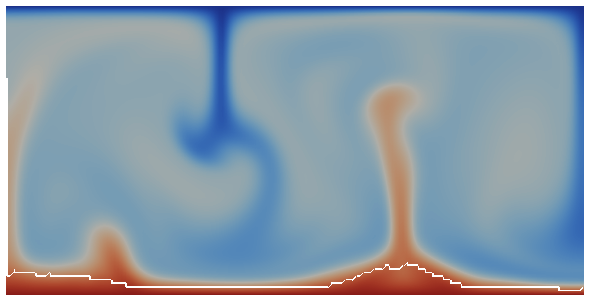
\includegraphics[width=0.45\columnwidth]{chapters/vynnytska/png/tmH.png} &
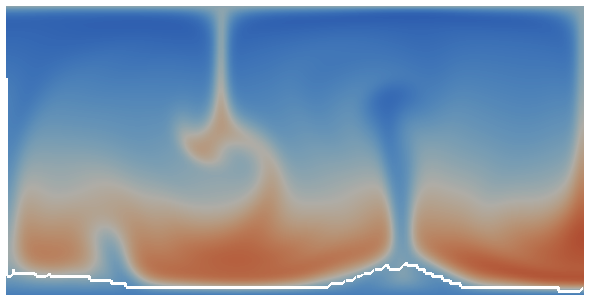
\includegraphics[width=0.45\columnwidth]{chapters/vynnytska/png/visH.png} \\ & $H$ \\
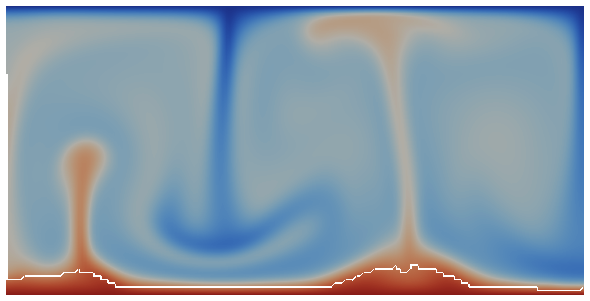
\includegraphics[width=0.45\columnwidth]{chapters/vynnytska/png/tmI.png} &
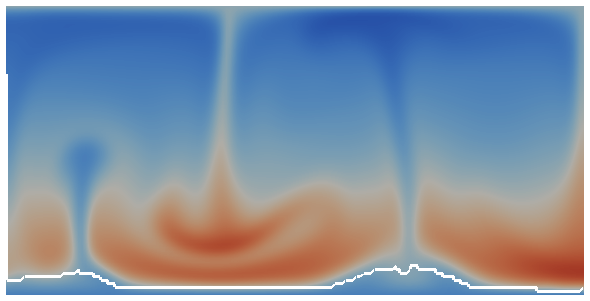
\includegraphics[width=0.45\columnwidth]{chapters/vynnytska/png/visI.png} \\ & $I$ \\
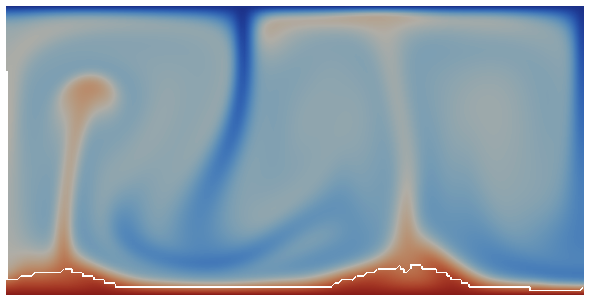
\includegraphics[width=0.45\columnwidth]{chapters/vynnytska/png/tmJ.png} &
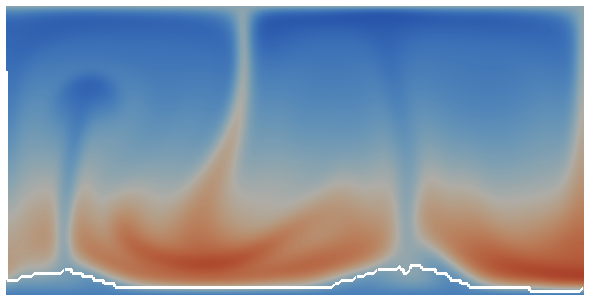
\includegraphics[width=0.45\columnwidth]{chapters/vynnytska/png/visJ.png} \\& $J$ \\
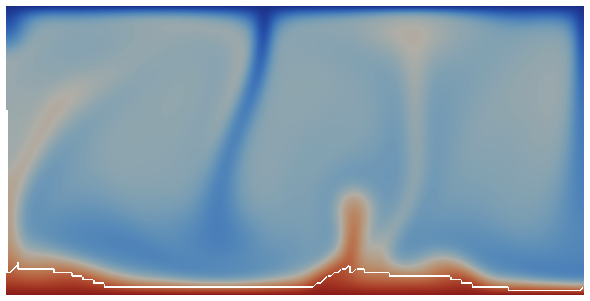
\includegraphics[width=0.45\columnwidth]{chapters/vynnytska/png/tmK.png} &
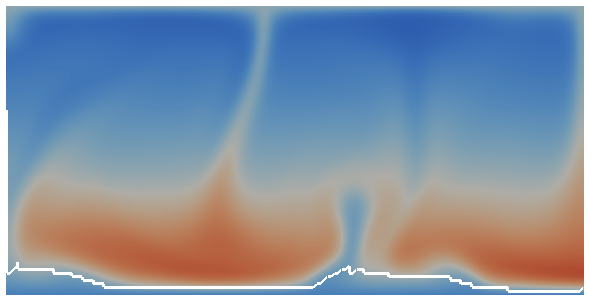
\includegraphics[width=0.45\columnwidth]{chapters/vynnytska/png/visK.png} \\& $K$ \\
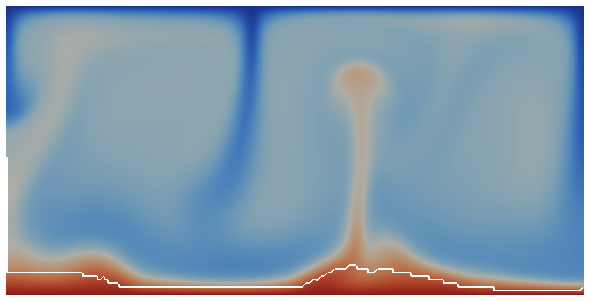
\includegraphics[width=0.45\columnwidth]{chapters/vynnytska/png/tmL.png} &
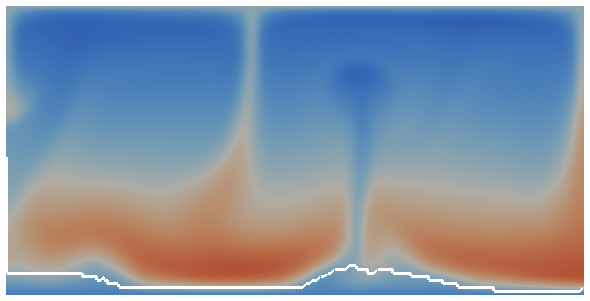
\includegraphics[width=0.45\columnwidth]{chapters/vynnytska/png/visL.png} \\& $L$ \\
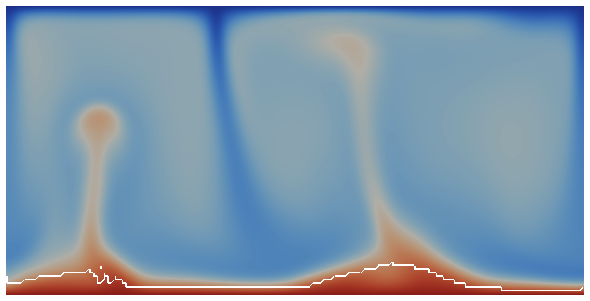
\includegraphics[width=0.45\columnwidth]{chapters/vynnytska/png/tmM.png} &
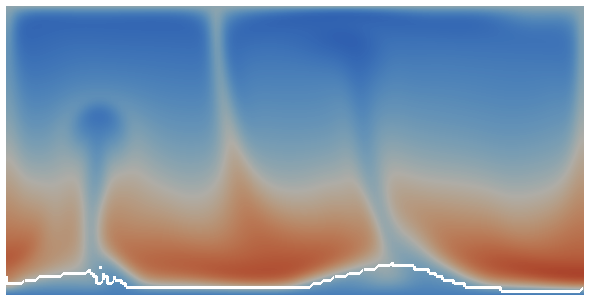
\includegraphics[width=0.45\columnwidth]{chapters/vynnytska/png/visM.png} \\& $M$ \\
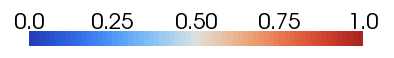
\includegraphics[width=0.45\columnwidth]{chapters/vynnytska/png/tmleg.png} &
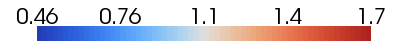
\includegraphics[width=0.45\columnwidth]{chapters/vynnytska/png/visleg.png}
\end{tabular}
\end{center}
\caption{Continued from Figure~\ref{vynnytska:fig:BG}, temperature and
  viscosity for points $H$ to $M$. During the stage $G$-$H$, a second
  slab forms and the two downwellings merge increasing the root-mean
  square velocity rapidly. From $H$, the downwelling is impeded by the
  higher viscosity at depth, reducing $u_{\mathrm{rms}}$ until $I$. Then a
  plume arising from the bottom left rises more rapidly through the
  lower viscosities of the upper mantle until $J$. Between $J$ and
  $K$, no new up- or downwellings occur, retarding the root-mean
  square velocity. From $K$ to $L$ a new plume increases the kinetic
  energy in the model, then pushes material laterally from underneath
  the top boundary layer until a slab begins to sink at the edge from
  $M$, increasing the velocity again.}
\label{vynnytska:fig:HM}
\end{figure}

%%------------------------------------------------------------------------------

\section{Discussion and concluding remarks}

The presented results show the mantle convecting with two distinct
chemical layers: plumes arise from atop piles on the denser bottom layer,
but are not compositionally distinct. The location of these piles is
initially set by the thermally dense slabs. Slabs collapsing into the
mantle drive the largest changes in the system energy, while plumes
drive smaller increases because their composition counteracts their
thermal buoyancy. The upwellings and downwellings react: slabs rapidly
sinking cause upwellings to form; the lateral motion of upwellings at
the top pushes and thickens the top layer, causing it to become unstable
and sink. As the system evolves, colder slab material builds up at the
bottom, increasing the viscosity of the lower mantle, while the reverse
happens in the upper mantle.

The simulation code for the convecting mantle has been included almost
in its entirety. We can conclude that the amount of code required
to implement such a problem within the FEniCS framework is quite
small. Moreover, the code for the variational problems closely matches
the mathematical formulation of the problems, and thus the complexity
of the code scales with the complexity of the numerical algorithm.
The numerical simulations presented here are spatially two-dimensional and
serve as a simplified model. Realistic three-dimensional simulations would
require taking advantage of the parallel, and possibly more sophisticated
adaptive, features of the FEniCS project. However, such would not require
significant additional problem-specific implementational effort, though
preconditioning would have to be carefully considered.

Tracking composition in the problem requires the solution of the
compositional advection-diffusion
equation~\eqref{vynnytska:eq:transdif}, creating difficulties for
standard field-based methods to solve because of sharp
discontinuities, often numerically smoothed by such methods.  Tracers
and marker chain approaches are often used to overcome this
problem~\citep{IsmailZadehTackley2010}. However, the approach
presented here allows us to represent compositional heterogeneities
because it employs discontinuous Galerkin methods, while a filtering
scheme minimizes the numerical smoothing error.

%%------------------------------------------------------------------------------
